\documentclass[12pt]{article}

\usepackage{subfigure}
\usepackage{pstricks}
\usepackage{pst-node}
\usepackage{graphicx}
\usepackage{authoraftertitle}
\usepackage[T1]{fontenc}
\usepackage{amsmath}
\usepackage{amsfonts}
\usepackage{amssymb}
\usepackage[lined,ruled,vlined,linesnumbered]{algorithm2e}
\usepackage{xspace,epsfig,url}
\usepackage{pst-plot,pstricks-add}

\newtheorem{theorem}{Theorem}
\newtheorem{definition}[theorem]{Definition}
%\newtheorem{remark}[theorem]{Remark}

\newenvironment{remark}
{% This is the begin code
\stepcounter{theorem}\vspace*{0.3cm}\noindent{\bf Remark} \arabic{theorem}.
}
{% This is the end code
}

\newtheorem{proposition}{Proposition}[section]
%\newtheorem{cor}[thm]{Corollary}

\newcommand{\comment}[2]{{\color{red}{\bf (#1: #2)}}}
\newcommand{\greedyAlgo}{\textsc{Greedy}}


\linespread{1.5}

\setlength{\leftmargin}{3.5cm}

\setlength{\topmargin}{2cm}

\setlength{\rightmargin}{2cm}

\newcommand{\ics}[2]{\langle #1, #2 \rangle}
%\newcommand{\ics}[2]{\frac{#1}{#2}}

\title{Algorithmic Optimization and Parallelization of Eppstein's Synchronizing Heuristic}

\author{Serta\c{c} Karahoda}

\date{}

\begin{document}

\maketitle
\thispagestyle{empty}
\vspace{1cm}

\begin{center}
Submitted to the Graduate School of Sabanc{\i} University \\
in partial fulfillment of the requirements for the degree of \\
Master of Science
\end{center}

\vspace{2cm}

\begin{center}
Sabanci University
\end{center}

\begin{center}
Augustus, 2017
\end{center}


\newpage
$ $
\thispagestyle{empty}
\newpage
$ $
\vspace{5cm}
\begin{center}
\copyright \hspace{0.1cm} \MyAuthor\space 2015

All Rights Reserved
\thispagestyle{empty}
\end{center}
\newpage

\begin{center}
\large
\MyTitle
\end{center}

\begin{center}
\MyAuthor

CS, Master's Thesis, 2017

Thesis Supervisor: H\"{u}sn\"{u} Yenig\"{u}n\\
Thesis Co--Supervisor: Kamer Kaya
\end{center}

\begin{center}
Keywords: ...
\end{center}

\begin{abstract}
...
\end{abstract}
\newpage

\begin{center}
\large
Eppstein'\i{}n S\i{}f\i{}rlama Sezgiselinin Algoritmik Eniyilemesi ve Paralelle\c{s}tirilmesi
\end{center}

\begin{center}
\MyAuthor

CS, Y\"{u}ksek Lisans Tezi, 2017

Tez Dan{\i}\c{s}man{\i}: H\"{u}sn\"{u} Yenig\"{u}n\\
Tez E\c{s}dan{\i}\c{s}man{\i}: Kamer Kaya
\end{center}

\begin{center}
Anahtar Kelimeler: ...
\end{center}

\begin{quote}
\begin{center}
{\bf \"{O}zet}
\end{center}

...

\end{quote}
\newpage
$ $
\vspace{2cm}
\begin{center}
\textbf{Acknowledgements}
\end{center}

%I would like to state my gratitude to my supervisor, H\"{u}sn\"{u} Yenig\"{u}n for everything he has done for me, especially for his invaluable guidance, limitless support and understanding. \\
%I would like to thank Hasan Ural and Guy-Vincent Jourdan for supporting this work with precious ideas and comments. \\
%I would like to thank my family for never leaving me alone. \\
%The financial support of Sabanci University is gratefully acknowledged. \\
%I would like to thank TUBITAK for the financial support provided.


\newpage
\tableofcontents

\newpage 
\listoffigures

\newpage
\listoftables



\newpage
\section{Introduction}
\label{sec:Intro}

\comment{Sertac}{Reset word'den bahsedecegim.}

\noindent
\comment{Sertac}{Intro'da FSM'den bahsedecegim.}

\noindent
\comment{Sertac}{cycle synchrop synchropl gibi algoritmalardan bahsedecegim.}

\newpage
\section{Preliminaries}
\label{sec:Preliminaries}
FSMs are mathematical abstractions for of real word systems. When an FSM gets an input, it moves from a state to another with an output. Since synchronization sequence consider only destination state, the output is not in the scope of this work. Therefore, we can consider FSMs are as automata with simple transaction function without an output.

When an {\em automaton} is complete and deterministic, it is defined by a triple $A=(S, \Sigma, \delta)$  where $S = \{1, 2, \ldots, n\}$ is a finite set of $n$ states, $\Sigma$ is a finite alphabet consisting of $p$ input symbols (or simply {\em letters}). $\delta : S \times \Sigma \rightarrow S$ is a transition function. If the automaton $A$ is at a state $s$ and if an input $x$ is applied, then $A$ moves to the state $\delta(s,x)$. Figure~\ref{fig:inv} shows an example automaton $A$ with 4 states and 2 inputs using graphical notation.\looseness=-1

\begin{figure}[h]
\centering
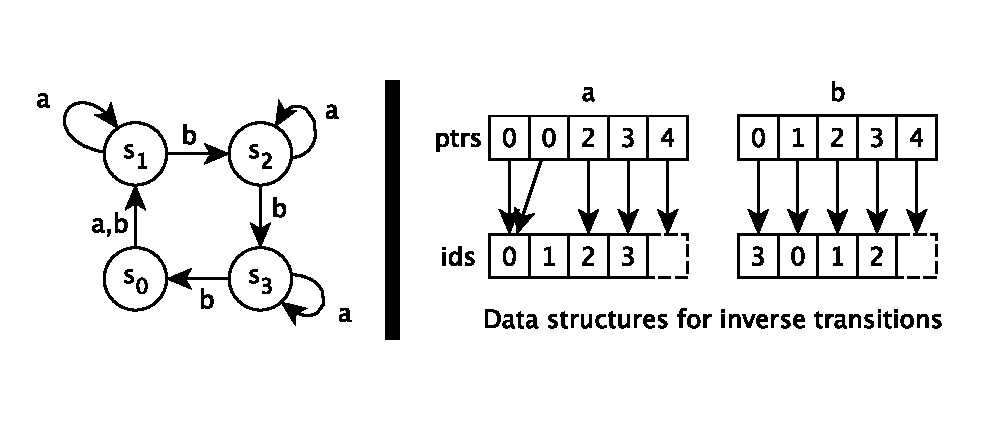
\includegraphics[width=0.7\textwidth]{figs/inverse.pdf}
\caption{A synchronizable automaton $A$~(left), and the data structures we used to store and process
the transition function $\delta^{-1}$  in memory (see Section~... for the details). A synchronizing sequence for $A$ is $abbbabbba$. \comment{sertac}{caption cok uzun belki iki figure olarak ayri ayri anlatabiliriz}}
\label{fig:inv}
\vspace*{-3ex}
\end{figure}

An element of the set $\Sigma^\star$ is called an {\em input sequence} (or simply {\em word}). $|w|$ denotes the length of $w$, and $\varepsilon$ expresses the empty word. Transition function $\delta$ can be extended to a set of states and to a word in the usual way. With fact $\delta(s,\varepsilon)=s$, let a word $w \in \Sigma^\star$ and a letter $x \in \Sigma$, then $\delta(s,xw) = \delta(\delta(s,x),w)$. Likewise, for a set of states $S' \subseteq S$, transaction function is $\delta(S',w) = \{ \delta(s,w) | s \in S'\}$.

Inverse of the transaction is also a well defined function. $\delta^{-1}(s,x)$ denotes the set of those states with a transition to state $s$ with input $x$. Formally, $\delta^{-1}(s,x) = \{ s' \in S | \delta(s',x)= s\}$.

Let $A=(S, \Sigma, \delta)$, $C \subseteq S$ and $C^{\langle 2 \rangle} = \{ \langle s_i, s_j \rangle | s_i,s_j \in C \}$ be set of multisets  with cardinality 2. For $\langle s_i, s_j \rangle \in C^{\langle 2 \rangle}$, if $s_i=s_j$ then it is called as \textit{singleton}, otherwise called as \textit{pair}. 

Let $C \subseteq S$ and $w \in \Sigma^*$, when cardinality of $\delta(C,w)$ is 1 then $w$ is \textit{merging sequence} for $C$ and $C$ is called \textit{mergeable}. If $C=S$, $w$ is called \textit{reset word} of automaton and the automaton is synchronizable.


\section{Eppstein's \greedyAlgo Algorithm}
In this section, Eppstein's \greedyAlgo is introduced. After that experiments and some analysis are shown. These analysis leads us to improve the speed of the algorithm.

\begin{proposition}
	\label{prop:synchronizable}
	An automaton $A=(S,\Sigma,\delta)$ is synchronizable iff for all  $s_i,s_j \in S$, there exists a merging sequence for $\{ s_i, s_j \}$.
\end{proposition}

The \greedyAlgo \space algorithm is one of the fastest algorithm among the reset word generating heuristics in the literature. Idea of the algorithm comes from proposition \ref{prop:synchronizable}. The algorithm uses merging sequences of pairs, in fact the shortest ones, to find a short reset word. Like most of algorithms mentioned in section \ref{sec:Intro}, \greedyAlgo \space has two main phases. At the first phase it finds the shortest merging sequences for all pairs. If there is a pair which is not mergeable, means that the automaton is not mergeable. Otherwise, the algorithm continues with second phase.

Merging sequence of pairs are stored in a function $\tau : S^{\langle 2 \rangle} \rightarrow \Sigma^\star$, which is called \textit{pairwise merging function (PMF)} for $A$. If $\{ s_i, s_j \}$ is mergeable, then $\tau(\{ s_i, s_j \})$ is the merging sequence, otherwise it is undefined. Note that PMF does not have to be unique, i.e. $\tau(\{ s_i, s_j \})$ may differ, however  $|\tau(\{ s_i, s_j \})|$ is unique. To find all shortest merging sequence, breath first search algorithm can be used. By using the inverse of transaction function and starting from $\langle s_i, s_i \rangle$ singletons, all mergeable pairs and their shortest merging sequences can be found iterative. Let $p=|\Sigma|$ and $n=|s|$, at worst case the algorithm traverse all edges, i.e. $p$ letters of each $n\cdot(n-1)$ pairs and $n$ singletons should be checked. Therefore the complexity of phase 2 is $O(pn^2)$. 

Algorithm \ref{algo:BFS} keeps track of most recent computed mergeable pairs , which is called \textit{frontier set (F)}. The level of frontier set refers the length of merging sequence. Since $\tau(\{ s_i, s_i \})=\epsilon$, singletons are defined as root level, level 0, of BFS algorithm. \textit{Remaining set (R)} is the set of pairs whose merging sequences are not computed yet. At each iteration of Algorithm \ref{algo:BFS} new frontier and remaining sets are computed for next level. 


\renewcommand{\baselinestretch}{0.9}
\begin{algorithm}
	\label{algo:BFS}
	\caption{Computing a PMF $\tau : S^{\langle 2 \rangle} \rightarrow \Sigma^\star$}
	\SetKwInOut{Input}{input}\SetKwInOut{Output}{output}
	\Input{An automaton $A=(S,\Sigma,\delta)$}
	\Output{A PMF $\tau : S^{\langle 2 \rangle} \rightarrow \Sigma^\star$}
	
	%compute the reverse automaton ${A}^{-1} = (S,\Sigma,\delta^{-1})$ of $A$;\\
	\lForEach{singleton $\langle s,s \rangle \in S^{\langle 2 \rangle}$}{$\tau(\langle s,s \rangle) = \varepsilon$}
	\lForEach{pair $\langle s_i,s_j \rangle \in S^{\langle 2 \rangle}$}{$\tau(\langle s_i,s_j \rangle) = \mbox{\em undefined}$}
	
	$F \longleftarrow \{ \langle s,s\rangle | s \in S \}$; \tcp{all singletons of $S^{\langle 2 \rangle}$}
    $R \longleftarrow \{ \langle s_i,s_j\rangle | s_i,s_j \in S \wedge s_i \neq s_j \}$; \tcp{all pairs of $S^{\langle 2 \rangle}$}
	\While{$R$ is not empty and $F$ is not empty}
	{
		$F,R,\tau \longleftarrow \mbox{BFS\_step}(A,F,R,\tau)$;\\
	}
\end{algorithm}
\renewcommand{\baselinestretch}{1}

Let a pair $\langle s_i,s_j \rangle \in S^{\langle 2 \rangle}$, if merging sequence of the pair is undefined and when a letter $x \in \Sigma$ is applied to the pair, resulting pair has merging sequence $w \in \Sigma^*$, then $\tau(\langle s_i,s_j \rangle) = x \cdot w$. Thanks to inverse of transaction function, Algorithm \ref{algo:BFS-step-F2R} computes the new frontier set from the most recent frontier set. At line 3-4, algorithm searches pairs which can reach the pairs of frontier set by applying one letter. If the merging sequence of found pair is not defined, then the algorithm defines it. Since the algorithm finds the remaining set from the frontier set, it is called \textit{frontier to remaining (F2R)}. 

\renewcommand{\baselinestretch}{0.9}
\begin{algorithm}
	\label{algo:BFS-step-F2R}
	\caption{{BFS\_step (F2R)}}
	
	\SetKwInOut{Input}{input}\SetKwInOut{Output}{output}
	\Input{An automaton $A=(S,\Sigma,\delta)$, the frontier $F$, the remaining set $R$, $\tau$}
	\Output{The new frontier $F'$, the new remaining set $R'$, and updated function $\tau$}
	
	$F' \longleftarrow \emptyset$;\\
	\ForEach{$ \langle s_i,s_j \rangle \in F$}
	{
		\ForEach{$x \in \Sigma$}
		{
			\ForEach{$\langle s'_i,s'_j\rangle$ such that $s'_i \in \delta^{-1}(s_i,x)$ and $s'_j \in \delta^{-1}(s_j,x)$}
			{
				\If(\tcp*[h]{$\langle s'_i,s'_j\rangle \in R$}){$\tau(\langle s'_i,s'_j\rangle)$ is undefined}
				{
					$\tau(\langle s'_i,s'_j\rangle) \longleftarrow x \tau(\langle s_i,s_j \rangle)$;\\
					$F' = F' \cup \{ \langle s'_i,s'_j\rangle  \} $;\\
				}
			}
		}
	}
	let $R'$ be $R \setminus F'$;
\end{algorithm}
\renewcommand{\baselinestretch}{1}

When first phase is completed, algorithm \ref{algo:greedy} checks the automata is synchronizable or not in $O(n^2)$ (line 2,3). After that it finds reset word iterative. it initialize the \textit{set of active states (C)} as set of all states and the reset word as empty word. At each iteration it selects the shortest merging sequence of all active pairs; appends it to reset word; finally updates the set of active states with applying the selected merging sequence. This operation repeats until only one active state left. At each iteration, merging sequence is applied, so the cardinality of $C$ decreases. Therefore iteration repeats at most $n$ times. At line 7 apply minimum operation among active pairs which is $O(n^2)$. Line 8 takes constant time. the complexity of computation line 9 is $O(n^?)$. Thus the phase 2 takes $O(n^?)$ and algorithm \ref{algo:greedy} requires $O(pn^2 + n^?)$ time.\comment{sertac}{mailde yazdigima gore revize etmek gerek.}

\renewcommand{\baselinestretch}{0.9}
\begin{algorithm}
	\label{algo:greedy}
	\caption{Eppstein's \textsc{Greedy} Algorithm}
	
	\SetKwInOut{Input}{input}\SetKwInOut{Output}{output}
	\Input{An automaton $A=(S,\Sigma,\delta)$}
	\Output{A reset word $\Gamma$ for $A$ (or fail if $A$ is not synchronizable)}
	
	%{--- Phase 1 ---}
	compute a PMF $\tau$ using Algorithm~\ref{algo:BFS}\;
	\If{there exists a pair $\langle s_i,s_j \rangle$ such that  $\tau(\langle s_i,s_j \rangle)$ is undefined}
	{
		report that $A$ is not synchronizable and exit;	
	}

	
	%{--- Phase 2 ---}
	$C = S$; \tcp{$C$ will keep track of the current set of states}
	$\Gamma = \varepsilon$; \tcp{$\Gamma$ is the synchronizing sequence to be constructed}
	
	\While(\tcp*[h]{we have two or more states yet to be merged}){$|C| > 1$}
	{
		find a pair $\langle s_i,s_j \rangle \in C^{\langle 2 \rangle}$ 
		with minimum $|\tau(\langle s_i,s_j \rangle)|$ among all pairs 
		in $C^{\langle 2 \rangle}$;\\
		
		
		$\Gamma = \Gamma \; \tau(\langle s_i,s_j \rangle)$;\\
		$C = \delta(C,\tau(\langle s_i,s_j \rangle))$;
	}
\end{algorithm}
\renewcommand{\baselinestretch}{1}

For small alphabet size and large number of states, second phase dominates the first phase in theory. However, experiments shows the contrary. Section \ref{sec:greedy-analysis} focuses on experiment results of \greedyAlgo and analysis of these experiments. \comment{sertac}{Biraz informal oldu sanki ama emin de olamadim}


\subsection{Analysis on \greedyAlgo}
\label{sec:greedy-analysis}

\newpage
\bibliographystyle{plain}
\bibliography{thesis}

\end{document}


